\documentclass[pdftex,a4paper,12pt,twoside,titlepage,italian,openright]{article}
\usepackage[italian]{babel}
\usepackage[utf8]{inputenc}
\usepackage{fancyhdr,graphicx}
\usepackage[hmargin=2cm,vmargin=2cm,a4paper]{geometry}
\usepackage{hyperref}
\usepackage{xcolor}
\pagestyle{fancy}
\lhead{\scshape Curriculum Vitae}
\rhead{\itshape Mauro Donadeo}
\rfoot{\footnotesize pag. \thepage}
\cfoot{}
\lfoot{{\footnotesize Aggiornato al: }\today}
\renewcommand{\headrulewidth}{.5pt}
\renewcommand{\footrulewidth}{.5pt}
%\renewcommand{\LettrineFontHook}{\color[gray]{0.5}}
\renewcommand*\familydefault{\sfdefault}
\renewcommand*\labelitemi{$\textcolor{black!30}{\bullet}$}
%\definecolor{listings-comment-color}{RGB}{20,0,0}

\begin{document}
\vspace*{.2cm}
\begin{center}
\rule{.8 \textwidth}{1pt}\\[5pt]
\begin{minipage}{.55\textwidth}
	\LARGE\textbf{Mauro Donadeo}\\[20pt]
	\footnotesize Via Isonzo 136/7 \\ 
	35143 - Padova (PD)\\
	email: \texttt{mauro.donadeo@gmail.com}\\
	\footnotesize n. Tel: +393467846243\\
	\footnotesize Nazionalità: Italiana\\
	\footnotesize Stato civile: Celibe\\
\end{minipage}
\begin{minipage}{.25\textwidth}
	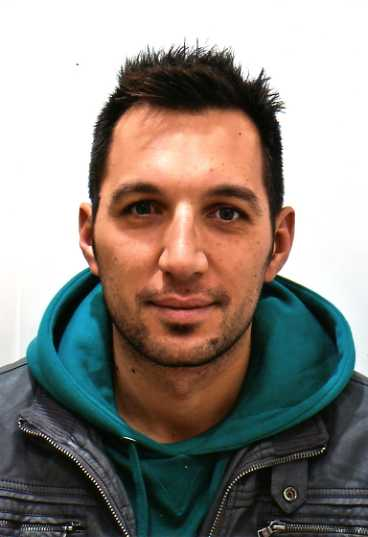
\includegraphics[width=\textwidth]{io.jpg}
\end{minipage}\\[5pt]
\rule{.8 \textwidth}{1pt}
\end{center}
\section*{Posizione attuale:}
	Contratto Co.Co.Co. per  lo sviluppo di un sistema di riconoscimento di gesture, acquisendo le immagini attraverso le camere
	del Microsoft Kinect; presso l'Univesità degli Studi di Padova al Dipartimento di Psicologia Generale. Il sistema è stato 
	sviluppato in C++ utilizzando le librerie OpenGL e OpenNi, le animazioni sono state riprodotte in Unity3D. Questo sistema è 
	stato sviluppato all'interno del progetto europeo CEEDs. 
\section*{Istruzione}
\begin{itemize}
	\item Laurea Magistrale in Ingegneria Informatica (Università degli Studi di Padova, Ottobre 2011).
	Titolo tesi: {\itshape Creazione di un sistema di videoconferenza 3D basato sul sensore MS Kinect}
	\item Laurea Triennale in Ingegneria Informatica (Università degli Studi di Padova, Aprile 2008). 
	Titolo tesi: {\itshape Realizzazione di un simulatore elementare del sistema robotico Lego Nxt
	in Java}
	\item Diploma Capo-tecnico Informatico (I.T.I.S. A. Meucci di Casarano (LE), 2004)
\end{itemize}
\section*{Esperienze all'estero}
\begin{itemize}
	\item 4th CEEDs meeting Londra (Febbraio 2012).
	\item Erasmus presso FIB - Facultat d’Inform`tica de Barcelona (a.a. 2009/2010)
\end{itemize}
\section*{Esperienze Professionali}
\begin{itemize}
	\item Docente Corso C.A.R (Corso Avananzato per la Ricerca) dal titolo ``Basi di Java''.
	Presso l'Univesità degli Studi di Padova - Dipartimento di Psicologia Generale
	\begin{itemize}
		\item Periodo Marzo-Aprile 2012;
		\item durata del corso 25 ore.
	\end{itemize}
	\item Web Designer presso Simnumerica S.r.l.
	\begin{itemize}
		\item dal Novembre 2011 al Dicembre 2011
		\item Creazione della pagina web dell'azienda. Principale occupazione: creazione del modulo di 
		iscrizione, news slider, e sistema di trouble ticketing.
	\end{itemize}
	\item Assistente informatico presso l'ufficio certificazione offerta didattica - SID.
	Presso: Università degli Studi di Padova
	\begin{itemize}
		\item Dal 01-09-2008 al 31-09-2009 
		\item Bonifica dati della base dati dell'Università, area didattica, prendendo come 
		modello i dati provenienti dal ministero.
		\item Creazione di una piccola applicazione web per il controllo delle attività didattiche
		per la generazione del \textit{diploma supplement}.
	\end{itemize}
	\item Assistente informatico presso l'Ufficio Tecnico e Coordinamento Reti. Presso:
	Regione del Veneto
	\begin{itemize}
		\item Dal Dicembre 2007 al Agosto 2008
		\item Progettazione e creazione del portale {\texttt overnetwork.it} basato sul {\textit cms Joomla}
		ed in particolare: creazione di un sistema di \textit{trouble ticketing} con conseguente 
		invio di notifiche tramite mail. Creazione di un nuovo sistema di \textit{profiling}
		degli utenti differente da quello previsto dalla piattaforma Joomla
	\end{itemize}
	%\item Portalettere per vari periodi presso i comuni di Cittadella (PD) e Campodarsego (PD).
\end{itemize}
\section*{Conoscenze informatiche:}
\begin{itemize}
	\item \textbf{S.O.:} Gnu/Linux conoscenza 	che va dall'installazione alla configurazione. Conoscenza anche dei vari 
	sistemi operativi Microsoft.
	\item \textbf{Programmazione: }:
	\begin{itemize}
	\item C/C++/C\#(anche con Microsoft Visual Studio 2010)
	\item Java
	\item Php MySql.
	\end{itemize}
	\item \textbf{Altro: }
	\begin{itemize}
	\item librerie per la {\itshape computer vision}: Directx10, OpenNI, OpenGL, OpenCV;
	\item sviluppo software su sistemi di acquisizione stereo e MS Kinect;
	\item Unity 3D Game Engine
	\item vim, Matlab, pacchetto Office, NXC, \LaTeX
	\end{itemize}
\end{itemize}
\section*{Conoscenze linguistiche:}
\begin{itemize}
	\item \textbf{Italiano:} madrelingua;
	\item \textbf{Inglese:} scolastico in writing e listening, buono nel reading.
	\item \textbf{Spagnolo:} ottima conoscenza sia scritta che parlata.
\end{itemize}
\section*{Interessi personali: }
\begin{itemize}
	\item Informatica in generale, editing video e immagini
	\item Sport: pratico nuoto e bicicletta, saltuariamente gioco a calcetto;
	\item Libri possibilmente in spagnolo per mantenere la conoscenza della lingua.
\end{itemize}
\vfill
Ai sensi del D. Lgs n. 196/2003 autorizzo al trattamento dei miei dati personali.
\vspace{1cm}
\end{document}
